\appendix
\section{Appendix}

\subsection{K-Nearest Neighbors (KNN)} \label{appendix:knn}
K-Nearest Neighbors (KNN) is a non-parametric, instance-based machine learning algorithm used for classification and regression tasks. Given a data point, KNN identifies the \(k\) nearest data points in the feature space based on a distance metric, commonly the Euclidean distance. For classification, the algorithm assigns the class most frequently occurring among the \(k\) neighbors. For regression, it predicts the average value of the neighbors. The choice of \(k\) significantly influences the model's performance, with smaller values leading to higher variance and larger values reducing sensitivity to noise. Formally, the Euclidean distance between two points \(\mathbf{x}_i\) and \(\mathbf{x}_j\) is defined as:

\[
d(\mathbf{x}_i, \mathbf{x}_j) = \sqrt{\sum_{l=1}^{n} (x_{il} - x_{jl})^2}
\]

where \(n\) is the number of features. The algorithm is simple but powerful, especially for low-dimensional data. For further details, read \cite{knn_model_based}.

\subsection{Kernel Density Estimation (KDE)} \label{appendix:kde}
Kernel Density Estimation (KDE) is a non-parametric method used to estimate the probability density function (PDF) of a random variable. Unlike histograms, KDE provides a smooth, continuous curve to describe the data distribution.

The KDE is defined as:
\[
\hat{f}(x) = \frac{1}{n h} \sum_{i=1}^{n} K\left(\frac{x - x_i}{h}\right)
\]
where:
\begin{itemize}
    \item \(\hat{f}(x)\): Estimated density at point \(x\).
    \item \(n\): Number of data points.
    \item \(h\): Bandwidth, controlling smoothness.
    \item \(K(\cdot)\): Kernel function, commonly Gaussian:
    \[
    K(u) = \frac{1}{\sqrt{2\pi}} e^{-\frac{u^2}{2}}
    \]
\end{itemize}

Each data point \(x_i\) contributes a kernel to the estimate. The bandwidth \(h\) determines the width of the kernels:
\begin{itemize}
    \item \textbf{Small \(h\)}: Produces a highly detailed density estimate but may overfit.
    \item \textbf{Large \(h\)}: Results in a smoother curve but may overlook finer details.
\end{itemize}

KDE is commonly used for data visualization to understand distributions and detect patterns like peaks or multimodality.
\cite{parzen1962}

\subsection{Tables}
\label{appendix:table}

\begin{figure}[H]
    \centering
    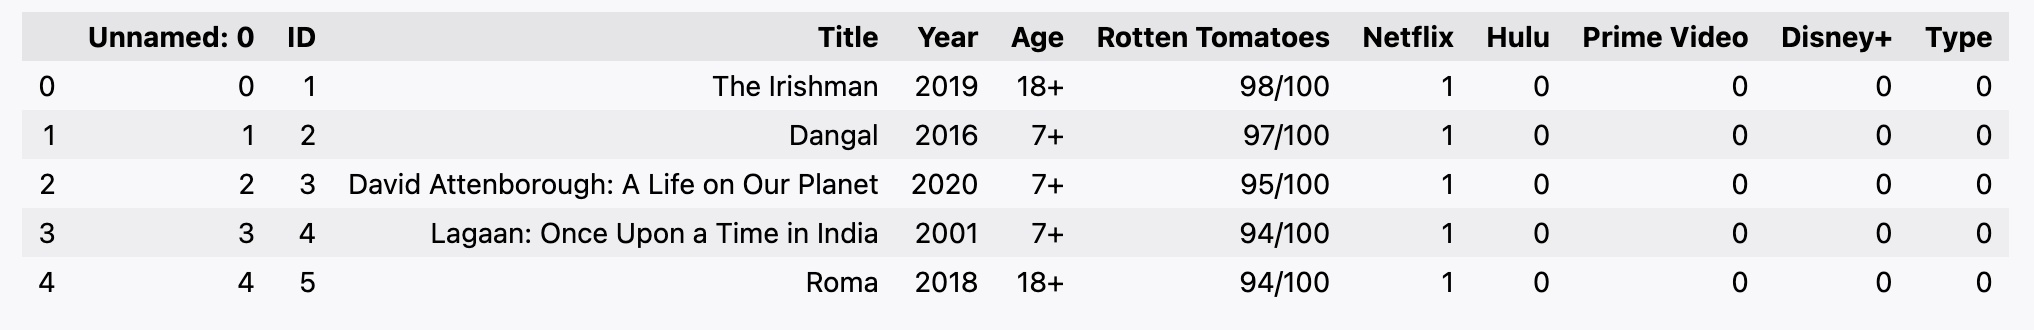
\includegraphics[width=1\textwidth]{head.png}
    \caption{First 5 Records of the Dataset}
    \label{fig:datatable}
\end{figure}

\subsection{Box Plot} \label{appendix:box_plot}
A box plot, or whisker plot, visualizes a dataset's distribution, showing its central tendency, spread, and outliers \cite{mcgill1978boxplots}.

\begin{enumerate}
    \item \textbf{Median (\(Q2\))}: 
    The midpoint of the dataset, dividing it into two equal halves:
    \[
    Q2 = 
    \begin{cases} 
    x_{\left(\frac{n+1}{2}\right)} & \text{if } n \text{ is odd} \\
    \frac{x_{\left(\frac{n}{2}\right)} + x_{\left(\frac{n}{2}+1\right)}}{2} & \text{if } n \text{ is even}.
    \end{cases}
    \]
    \item \textbf{Interquartile Range (IQR)}:
    The range of the middle 50\% of the data:
    \[
    IQR = Q3 - Q1
    \]
    where \(Q1\) and \(Q3\) are the 25th and 75th percentiles, respectively.

    \item \textbf{Whiskers}:
    Extend to the smallest and largest values within 1.5 times the IQR:
    \[
    \text{Lower whisker} = \max(\min(\text{data}), Q1 - 1.5 \times IQR)
    \]
    \[
    \text{Upper whisker} = \min(\max(\text{data}), Q3 + 1.5 \times IQR)
    \]

    \item \textbf{Outliers}:
    Data points beyond the whiskers:
    \[
    \text{Outliers} < Q1 - 1.5 \times IQR \quad \text{or} \quad \text{Outliers} > Q3 + 1.5 \times IQR.
    \]
\end{enumerate}

Box plots help identify the \textbf{median} (central tendency), \textbf{IQR} (spread), and \textbf{outliers} (anomalies).

\subsection{Shapiro-Wilk Test} \label{appendix:shapiro}
The Shapiro-Wilk test evaluates whether a dataset follows a normal distribution. It calculates a test statistic based on the correlation between the data and their corresponding normal scores. The test statistic \(W\) is defined as:

\[
W = \frac{\left( \sum_{i=1}^{n} a_i x_{(i)} \right)^2}{\sum_{i=1}^{n} (x_i - \bar{x})^2}
\]

Where:
\begin{itemize}
    \item \(x_{(i)}\): Ordered sample values (from smallest to largest).
    \item \(a_i\): Weights derived from the expected values of the order statistics of a standard normal distribution.
    \item \(\bar{x}\): Sample mean.
    \item \(n\): Number of observations.
\end{itemize}

A \textbf{p-value $<$ 0.05} suggests that the data significantly deviate from normality. This test is particularly effective for small sample sizes. \cite{shapiro1965}

\subsection{Kolmogorov-Smirnov Test} \label{appendix:kolmogorov}
The Kolmogorov-Smirnov (K-S) test compares the empirical cumulative distribution function (ECDF) of a dataset, \(F_n(x)\), to a specified theoretical cumulative distribution function (CDF), \(F(x)\). The test statistic \(D\) is defined as:

\[
D = \max | F_n(x) - F(x) |
\]

Where:
\begin{itemize}
    \item \(F_n(x)\): Empirical CDF of the sample.
    \item \(F(x)\): Theoretical CDF of the specified distribution (e.g., normal).
\end{itemize}

A \textbf{p-value $<$ 0.05} indicates that the data do not follow the specified distribution. The test is sensitive to differences in both the center and the tails of the distribution. \cite{smirnov1948}

\subsection{Mann-Whitney U Test} \label{appendix:mann}
The \textbf{Mann-Whitney U test} is a non-parametric test used to determine whether there is a significant difference between the distributions of two independent groups. Unlike the t-test, it does not assume normality or equal variances. The test ranks all data points from both groups together and then evaluates whether the ranks of one group are systematically higher or lower than the other. It is particularly useful for comparing medians or when the data are ordinal or not normally distributed. \cite{mann1947}

\subsection{P-value} \label{appendix:pvalue}
The \textbf{p-value} is a measure used in statistical hypothesis testing to quantify the evidence against the null hypothesis (\(H_0\)). It represents the probability of observing a test statistic as extreme as, or more extreme than, the one observed, assuming that \(H_0\) is true.

Mathematically, the p-value is defined as:
\[
p = P(T \geq T_{\text{obs}} \mid H_0)
\]
where:
\begin{itemize}
    \item \(T\) is the test statistic.
    \item \(T_{\text{obs}}\) is the observed value of the test statistic.
    \item \(H_0\) is the null hypothesis.
\end{itemize}

A smaller p-value (e.g., \(p < 0.05\)) indicates stronger evidence against the null hypothesis, leading to its rejection. Conversely, a larger p-value suggests insufficient evidence to reject \(H_0\). \cite{pearson1900}
